%%%%%%%%%%%%%%%%%%%%%%%%%%%%%%%%%%%%%%%%%%%%%%%%%%%%%%%
% A template for Wiley article submissions.
% Developed by Overleaf. 
%
% Please note that whilst this template provides a 
% preview of the typeset manuscript for submission, it 
% will not necessarily be the final publication layout.
%
% Usage notes:
% The "blind" option will make anonymous all author, affiliation, correspondence and funding information.
% Use "num-refs" option for numerical citation and references style.
% Use "alpha-refs" option for author-year citation and references style.

% \documentclass[alpha-refs]{wiley-article}
\documentclass[num-refs]{wiley-article}

% Add additional packages here if required
\usepackage{siunitx}

% Update article type if known
\papertype{Original Article or Review?}
% Include section in journal if known, otherwise delete
\paperfield{Methods \& Resources}

\title{Batch effects in large-scale proteomics studies: diagnostics and correction}

% Include full author names and degrees, when required by the journal.
% Use the \authfn to add symbols for additional footnotes and present addresses, if any. Usually start with 1 for notes about author contributions; then continuing with 2 etc if any author has a different present address.
\author[1, 2, 3]{Jelena Čuklina}
\author[1]{Chloe Lee}
\author[1]{Evan G. Williams}
\author[1]{Tatjana Sajic}
\author[1\authfn{2}]{Ben C. Collins}
\author[3]{Maria Rodriguez-Martinez}
\author[2]{Varun Sharma}
\author[1, 4]{Patrick Pedrioli}
\author[1, 5]{Ruedi Aebersold}

% Include full affiliation details for all authors
\affil[1]{Institute of Molecular Systems Biology, ETH Zurich, Zurich, CH-8093, Switzerland}
\affil[2]{PhD Program in Systems Biology, University of Zurich and ETH Zurich, Zurich, CH-8057  Switzerland}
\affil[3]{IBM Zurich Research Laboratory, Rüschlikon, CH-8803, Switzerland}
\affil[4]{ETH Zürich, PHRT-MS, Zürich, Switzerland}
\affil[5]{Faculty of Science, University of Zurich, Zurich, Switzerland}

\corraddress{Ruedi Aebersold, Institute of Molecular Systems Biology, ETH Zurich, Zurich, CH-8093, Switzerland}
\corremail{aebersold@imsb.biol.ethz.ch}

\presentadd[\authfn{2}]{Department, Institution, City, State or Province, Postal Code, Country}

\fundinginfo{J.Č. was supported by funding from the European Union Horizon 2020 research and innovation program under grant agreement No 668858 and the Swiss State Secretariat for Education, Research and Innovation (SERI) under contract number 15.0324-2. P.P. was supported by SNF grant no. SNF IZLRZ3\_163911.}

% Include the name of the author that should appear in the running header
\runningauthor{Čuklina et al.}

\begin{document}

\maketitle

\begin{abstract}
Advances in mass spectrometry based proteomics have significantly increased sample throughput and sample to sample reproducibility to a degree that large-scale studies consisting of hundreds of samples are becoming routine. Increased sample numbers, however, come at the price of introducing batch effects, that decrease the power to identify the underlying biological variance. 

Here, we present step-by-step workflow for batch effects analysis in proteomics. This workflow allows to assess batch effects in a given dataset, select appropriate methods for their correction and control the quality of the correction. This workflow addresses mass-spectrometry specific issues, such as gradual MS signal deterioration, and batch-specific missingness. We propose solutions for both issues. Corresponding tools are freely accessible as R package "proBatch".

We demonstrate the workflow on three large-scale  proteomics datasets. Although applied to DIA proteomics, the principles described here are expected to be applicable to wide range of proteomic methods.

\keywords{Batch effects, Quantitative proteomics, Normalization}
\end{abstract}

\section{Introduction}
Recent advances in mass-spectrometry enabled fast and near-exhaustive identification and quantification of proteins in complex biological samples \cite{Schubert2017}. Quantitative robustness and sample throughput of techniques such as DIA/SWATH-MS allow to profile large sample cohorts with high quantitative accuracy \cite{Williams:2016aa, Liu2015, Sajic2018, Okada2016}.  

Consistent and accurate proteome profiling for large-scale studies, especially profiling patient cohorts, is particularly challenging. Obtaining sufficiently large dataset is associated with considerable logistic efforts: typically, multiple biomaterial handlers are involved, protein extraction and digestion is performed in batches that use different reagent lots, and the whole procedure takes a lot of time, as sample preparation cannot be completed in one day, and also the mass-spectrometric measurement requires days or weeks of instrument time. This introduces systematic technical variation known as the batch effect.

Batch effects can only be corrected if batch factors have been considered in experimental design, otherwise, the data can be biased beyond repair  \cite{Hu2005, Gilad2015}. At the stage of experimental design, the main goal is to prevent confounding of biological groups and technical factors, causing batch effects. Also, number of samples, ensuring sufficiently powered study has to be evaluated. For control of variability, replicates should be included into the study. Experimental design is a complex issue, spanning beyond the scope of this article, however, the reader can use previously published materials on the topic \cite{Oberg2009, Cuklina2020}. With careful experimental design, batch effects can be adjusted for, uncovering biological signal in the data.

The fundamental objective of the batch effect adjustment procedure is to make all measurements of samples comparable for a meaningful biological analysis (\cite{Leek:2010aa}) and to remove variance of non-biological origin (\cite{Bolstad2003}). Number of articles, dedicated to the topic is constantly increasing; new methods and packages are being published; tools performance has been compared (\cite{Luo2010, Chen:2011ac, Dillies:2013aa, Chawade:2014aa}). Some of these tools have been developed for transcriptomics (\cite{Johnson:2007aa, Sims:2008aa, Leek:2007aa, Benito2004, Dillies:2013aa}), certain could be ported to proteomics \cite{Lee:2019aa}. Others have been used in application to mass-spectrometry data (\cite{Karpievitch2012, Chawade:2014aa, Valikangas2018, Gregori2012}). Application of these tools, however, remains challenging. First, the sequence of steps is often confused. Most prominent example being confusion of terms “normalization” and “batch correction”, while they represent different approaches to data transformation. Second, each tool published has been implemented independently, assuming variety of data input  and output formats, making analysis prone to errors or cumbersome to combine into pipelines. Third, mass-spectrometry based proteomics has unique batch-associated biases, such as gradual MS signal deterioration, that need new approaches for bias correction. Finally, it remains hard to determine that the data correction “worked” and the data has improved. Thus, quality control metrics need to be developed and included into the workflow. In this study, we propose a workflow, that addresses proteomics batch effects problem in a systematic way: we clarify the definitions, justify the choice of methods at each step, implement it into a tool called “proBatch”. It should be noted, that we do not provide an exhaustive comparison of existing tools, for which numerous articles have been published previously \cite{Lazar:2013aa, Chawade:2014aa, Cheng:2012aa}. We, however, indicate the principles that guide a choice of the method and provide tips for tool developers that are instrumental for their compatibility with other components of the workflow. We include the tools that we consider most universal in "proBatch" and illustrate each step using real-world large-scale proteomic data.

We use three large-scale DIA datasets to demonstrate the workflow. Some of the diagnostic, correction and quality approaches are universal, while others are dataset-specific. Dataset-specific steps depend sometimes on nature of the data (experimental design or expected heterogeneity). Which is why several datasets are essential to demonstrate the decision making along the workflow, as will be demonstrated in the next sections of this manuscript. Two of these datasets, that were published earlier (\cite{Collins2017, Sajic2018}) have been used as sources of “good practices” to develop the workflow, and define checkpoints, where dataset-specific decisions need to be made. The third dataset is new and is used as a test case, on which we could try the established and novel tools. This dataset features 375 mass-spectrometry runs measuring \~ 18000 peptidoforms of \~2100 proteins and is the largest in our collection, and also the most representative in terms of experimental design and batch factors that are likely to occur in large-scale mass-spectrometry based proteomics. We go along the workflow using this dataset, referring to other two datasets, where other desicions are likely to be made. We provide the code of the analysis for all three dataset, so that the steps described here could be applied by a wider community of researchers.

This paper is organised as follows: first, we describe the datasets, used to define and test the workflow. Next, we provide a brief overview of the workflow and define key terms for each step. We then expand each step, using the examples of Mouse Aging Study to illustrate them, and refer to other two datasets, when appropriate. We devote a specialized section to the problem of missing values in relation to batch effects and indicate the caution points related to missing value imputation. Aftern that we describe the "proBatch" tool and finish the manuscript with discussion of generalizability of the principles described to other methods or data acquision, in proteomics and beyond.. In conclusion, we summarize the information provided in previous sections and outline the expected developments in batch effects research.

\section{Addressing batch effects: the workflow}
\subsection{Workflow overview}
Most of the data, acquired with high-throughput technologies, including MS-proteomics, can not be used in statistical analysis or model learning directly. The procedure ensuring comparability of the samples is known as batch correction. This procedure can be separated into the sequence of steps, as shown in Figure~\ref{fig:batch_fig1_workflow} and explained in more detail below.  
\begin{figure}[bt]
	\center
	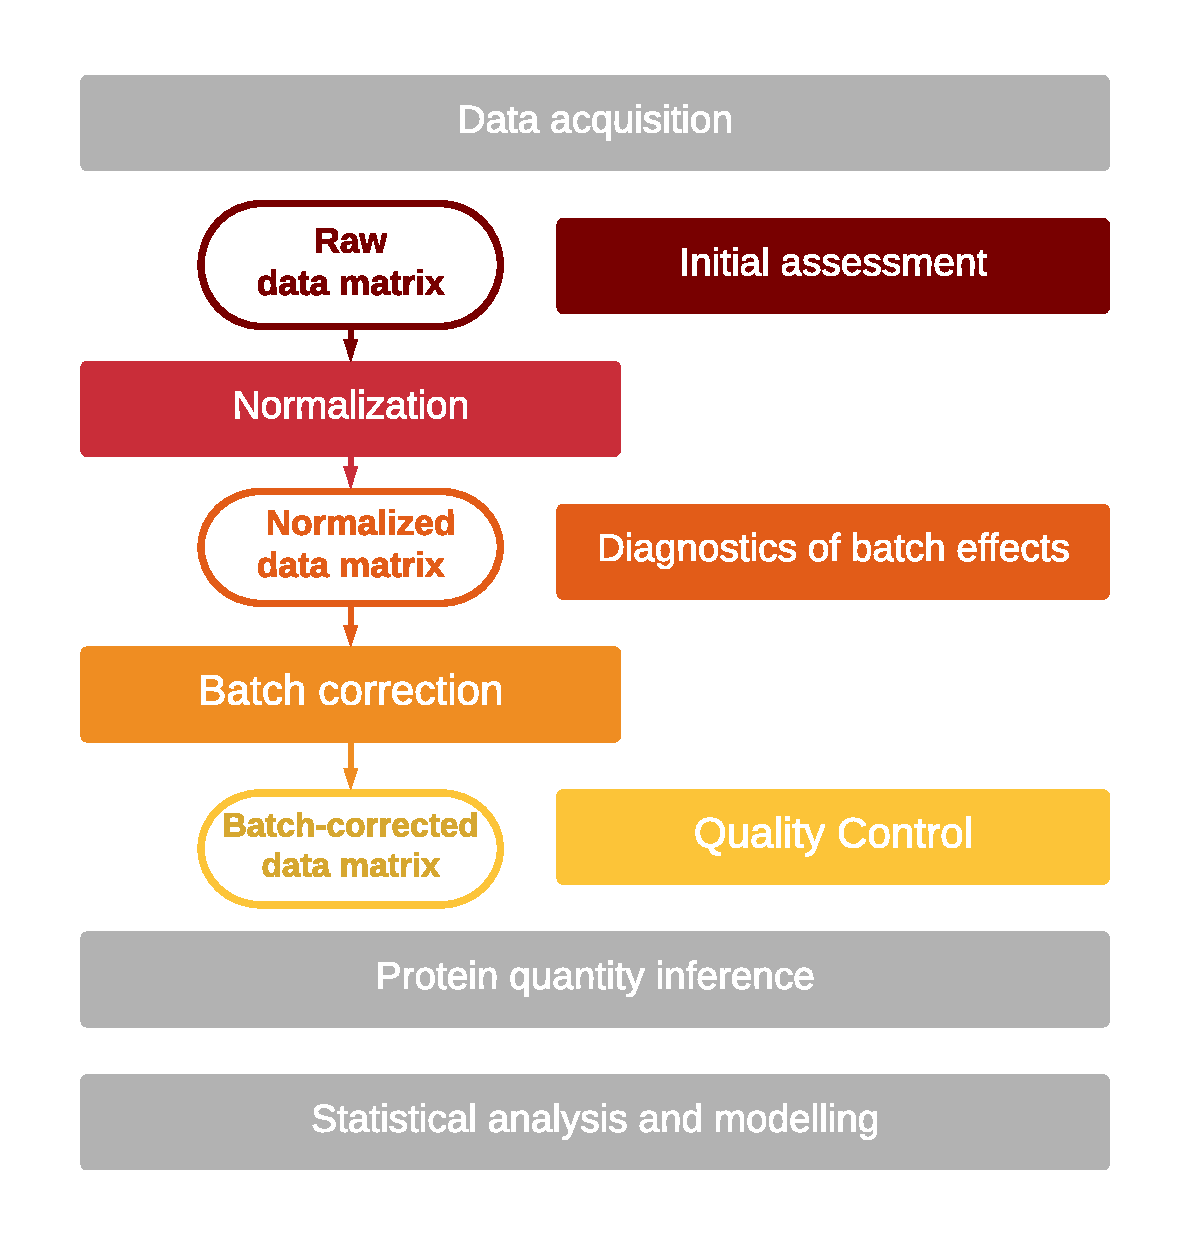
\includegraphics[width=6cm]{figures/Fig0_workflow_staircase}
	\caption[Batch effect correction workflow]
	{Batch effect processing workflow}
	\label{fig:batch_fig1_workflow}
\end{figure}

We suggest a five-step workflow to address batch effects in large-scale dataset. Initial assessment allows to evaluate whether batch effects are present in raw, unnormalized data and to select normalization procedure. Second, normalization brings all samples from the dataset to the common scale, typical methods of normalization being sample-wide quantile normalization and median normalization. Third step is diagnostics of batch effects in normalized data, with methods such as PCA, hierarchical clustering. This step determines whether further correction is required. If batch effects are still present in the data, a furter step of batch correction is required. Batch correction addresses feature-specific biases, commonly addresses with tools like ComBat \cite{Johnson:2007aa} or feature-specific mean/median centering. Finally, quality control ensures that the data has been improved by correction: biases have been reduces while meaningful signal has been retained. In the next sections, we discuss each step of the workflow in more detail, illustrating it with examples from three large-scale proteomic datasets.

\subsection{Data processing preceding the workflow} 
This workflow takes quantitative data matrix as an input. Thus, it is assumed that the workflow starts with the data matrix, for which peptide-spectrum matching, and FDR control are completed. We strongly suggest to perform the protein quantification after the batch effects correction, as this procedure alters the abundances of transition and peptide, and these abundances are critical for the protein quantity inference \cite{Clough:2012aa, Teo:2015aa}.  

Also, we suggest to keep all detected peptides, also non-proteotypic and the ones with multiple missing values. Keeping all measurements allows to better evaluate the distribution within each sample, which is critical for subsequent normalization and batch adjustment steps.

Data is assumed to be log-transformed, unless the variance stabilizing transformation \cite{Durbin2002} is used, as this normalization method has log-like transformation integrated into the normalization procedure.

\subsection{Adding Citations and a References List}

Please use a \verb|.bib| file to store your references. When using Overleaf to prepare your manuscript, you can upload a \verb|.bib| file or import your Mendeley, CiteULike or Zotero library directly as a \verb|.bib| file\footnote{see \url{https://www.overleaf.com/blog/184}}. You can then cite entries from it, like this: \cite{Gregori2012}. Just remember to specify a bibliography style, as well as the filename of the \verb|.bib|.

You can find a video tutorial here to learn more about BibTeX: \url{https://www.overleaf.com/help/97-how-to-include-a-bibliography-using-bibtex}.

This template provides two options for the citation and reference list style: 
\begin{description}
\item[Numerical style] Use \verb|\documentclass[...,num-refs]{wiley-article}|
\item[Author-year style] Use \verb|\documentclass[...,alpha-refs]{wiley-article}|
\end{description}

\subsubsection{Third Level Heading}
Supporting information will be included with the published article. For submission any supporting information should be supplied as separate files but referred to in the text.

Appendices will be published after the references. For submission they should be supplied as separate files but referred to in the text.

\paragraph{Fourth Level Heading}
% Here are examples of quotes and epigraphs.
\begin{quote}
The significant problems we have cannot be solved at the same level of thinking with which we created them.\endnote{Albert Einstein said this.}
\end{quote}

\begin{epigraph}{Albert Einstein}
Anyone who has never made a mistake has never tried anything new.
\end{epigraph}

\subparagraph{Fifth level heading}
Measurements should be given in SI or SI-derived units.
Chemical substances should be referred to by the generic name only. Trade names should not be used. Drugs should be referred to by their generic names. If proprietary drugs have been used in the study, refer to these by their generic name, mentioning the proprietary name, and the name and location of the manufacturer, in parentheses.

\begin{table}[bt]
\caption{This is a table. Tables should be self-contained and complement, but not duplicate, information contained in the text. They should be not be provided as images. Legends should be concise but comprehensive – the table, legend and footnotes must be understandable without reference to the text. All abbreviations must be defined in footnotes.}
\begin{threeparttable}
\begin{tabular}{lccrr}
\headrow
\thead{Variables} & \thead{JKL ($\boldsymbol{n=30}$)} & \thead{Control ($\boldsymbol{n=40}$)} & \thead{MN} & \thead{$\boldsymbol t$ (68)}\\
Age at testing & 38 & 58 & 504.48 & 58 ms\\
Age at testing & 38 & 58 & 504.48 & 58 ms\\
Age at testing & 38 & 58 & 504.48 & 58 ms\\
Age at testing & 38 & 58 & 504.48 & 58 ms\\
\hiderowcolors
stop alternating row colors from here onwards\\
Age at testing & 38 & 58 & 504.48 & 58 ms\\
Age at testing & 38 & 58 & 504.48 & 58 ms\\
\hline  % Please only put a hline at the end of the table
\end{tabular}

\begin{tablenotes}
\item JKL, just keep laughing; MN, merry noise.
\end{tablenotes}
\end{threeparttable}
\end{table}

\section*{acknowledgements}
Acknowledgements should include contributions from anyone who does not meet the criteria for authorship (for example, to recognize contributions from people who provided technical help, collation of data, writing assistance, acquisition of funding, or a department chairperson who provided general support), as well as any funding or other support information.

\section*{conflict of interest}
You may be asked to provide a conflict of interest statement during the submission process. Please check the journal's author guidelines for details on what to include in this section. Please ensure you liaise with all co-authors to confirm agreement with the final statement.

\printendnotes

% Submissions are not required to reflect the precise reference formatting of the journal (use of italics, bold etc.), however it is important that all key elements of each reference are included.
\bibliography{proteomics_thesis}

\graphicalabstract{example-image}{Please check the journal's author guildines for whether a graphical abstract, key points, new findings, or other items are required for display in the Table of Contents.}

\end{document}
